\chapter{Partikelrörelse i celler}

Partikelrörelse i cellers cytoplasma är något som länge fascinerat forskare inom området. En enkel modell som modellerar partikelrörelserna som klassisk brownsk rörelse kan inte förklara de observerade egenskaperna där en långsammare diffusion är ett av de mest tydliga exemplen. Andra modeller har tagits fram i avsikt att försöka förklara rörelsen men i dagsläget finns inte någon universell modell som kan beskriva rörelsen fullständigt. 

Detta kapitel presenterar inledningsvis tre möjliga förklaringsmodeller till partikelrörelsen:  Ornstein-Uhlenbeck-processen, CTRW och fBm som alla tre har kopplingar till klassisk brownsk rörelse. 

I denna studie undersöks om given data över partikelrörelse i jästceller har egenskaper, bland annat MSD och asphericity, som kan beskrivas av dessa modeller. Både teoretiska beräkningar och simuleringar används för att göra jämförelsen. Den stora skillnaden mellan CTRW och fBm är att CTRW är en icke-stationär process medan fBm är stationär, något som används för att avgöra deras relevans som förklaringsmodeller. \todo{O-U är stationär.}

Några av de viktigaste resultaten som presenteras i detta kapitel är att rörelsen verkar vara stationär och att rörelsen är minst lika isotrop som en Wienerprocess med identisk fördelningsfunktion för steg i x- och y-led. \todo{Här kan man fylla i det man tycker är relevant}



\subsubsection{Undersökt data}
Datan som studerats för partikelrörelse är samma som \cite{Midtveldt_etal2016} använde och utgörs av mätningar av positionen för fluorescerande partiklar i jästceller. Jästcellerna hade genmodifierats till att producera fluorescerande protein som lätt bildar kluster. Dessa kluster brukar vara av storleksordning 100--500\,nm, vilket kan jämföras med själva cellernas storlek på omkring 5\,\micro{m}.

Data för ett hundratal partiklar från olika jästceller ingick i mätserien, både för aktiva celler och celler som försatts i dvala med sänkt metabol aktivitet. Mätningen genomfördes med 100 bilder per sekund.



\section{Modeller för partikelrörelse i vätskor}

Till en första approximation skulle rörelsen för en partikel i en jästcells cytoplasma kunna beskrivas med klassisk brownsk rörelse. Partiklarna krockar där med mindre partiklar från omgivningen och rörelsen kan då beskrivas med en stokastisk gaussisk propagator~\cite{Einstein1905}
\begin{equation}
P(x,t)=\frac{1}{\sqrt{4\pi Dt}}\ee^{\nicefrac{-x^2}{4Dt}}
\end{equation} %Obs n=1 då endast en partikel följs
som utgörs av sannolikhetstätheten för partikelns förflyttning $x$ vid en given tid $t$, där konstanten $D$ är dess diffusionskonstant. Om partikeln betraktas som en sfär med radie $r$ nedsänkt i en vätska med dynamisk viskositet $\mu$ och absolut temperatur $T$ kan $D$ approximeras till~\cite{Einstein1905}
\begin{equation}
D=\frac{k_\text{B} T}{6\pi \mu r}.
\end{equation}
%Man betraktar då cytoplasman som en homogen vätska. %Denna teori bygger dock på att man har termisk jämvikt och att partiklar rör sig i en enbart viskös vätska, två kriterier som inte uppfylls i cytoplasman bland annat på grund av mitokondriernas energiutvinning.

Experiment\cite{Midtveldt_etal2016} har dock visat att diffusionen av partiklar i celler är fundamentalt långsammare än förväntat från klassisk brownsk rörelse. Det finns ett par verktyg man kan använda för att undersöka detta. Ett av dem är MSD. Som visades i avsnitt~\ref{sec:brown} är MSD:n för brownsk rörelse proportionell mot förlupen tid. Speciellt kan \eqref{eq:MSD_brown} skrivas om till
\begin{equation}
\ev{x(t)^2} \propto t,
\end{equation}
där $x(0)=0$. Vad \cite{Midtveldt_etal2016} då har funnit i tidigare studier är att exponenten på $t$ är lägre än~$1$, vilket tyder på att andra förklaringsmodeller kan behövas.


\subsection{Ornstein-Uhlenbeck-process}
En första utvidgning av modellen för brownsk rörelse fås genom att lägga till en återförande term som drar partikeln mot någon medelpunkt. Detta är en så kallad Ornstein-Uhlenbeck-process
\begin{equation}\label{eq:SDE_o-u}
\pd_t x = -\gamma ( x-\bar{x} ) + \pd_t W,
\end{equation}
där $\gamma$ är en tidsskala som styr hur hårt bunden partikeln är till medelpositionen $\bar{x}$, och $\pd_t W$ är den stokastiska drivningen av partikeln som uppfyller $\ev{\pd_t W}=0$ och $\ev{\pd_t W(t)\pd_t W(t')} = \sigma^2\delta(t-t')$. Detta är en inte helt orimlig modell eftersom en partikel i en cell rimligtvis inte kan vandra hur långt som helst. Typiskt kommer en partikel att tränga ihop cytoplasmans beståndsdelar i den riktning som den rör sig åt, vilket leder till en återförande kraft.

Med \eqref{eq:SDE_o-u} och metoderna från avsnitt~\ref{sec:brown} kan modellens autokorrelation och MSD härledas. Autokorrelationen i gränsen mot ett stationärtillstånd ($\gamma t\gg 1$) blir då i en dimension
\begin{equation}\label{eq:COV_o-u}
\ev{x(t)x(t+\Delta{t})} \approx \frac{\sigma^2}{2\gamma} \ee^{-\gamma\Delta{t}},
\end{equation}
där $\bar{x}$ har satts till 0. Vidare kan också MSD beräknas; med $\Delta{t}=\abs{t-t'}$ erhålls
\begin{equation}\label{eq:MSD_o-u}
\ev{\Big(x(t)-x\big(t'\big) \Big)^2} 
\approx \frac{\sigma^2}{\gamma} \left( 1-\ee^{-\gamma \Delta{t}} \right).
\end{equation}




\subsection{Continuous Time Random Walk (CTRW)}
En möjlig förklaringsmodell för anomal transport i celler utgörs av CTRW (Continuous-Time Random Walk)~\cite{Hofling&Franosch2013}. Här beskrivs rörelsemönstret av att partiklarna under majoriteten av tiden sitter bundna till olika nätliknande strukturer för att sedan plötsligt ta sig vidare till en ny position efter en viss tid. Partiklarnas steglängder samt väntetider mellan steg är stokastiska variabler och för härledning av partikelns egenskaper se bilaga~\ref{app:CTRW}. Den stora skillnaden mellan en CTRW modell och enkel slumpvandring är att väntevärdet av tiden mellan två steg kan vara odefinierad för en CTRW modell. I dessa fall kan följande fördelningsfunktion för väntetiderna användas
\begin{equation}
\psi(t) \sim \frac{1}{t^{\alpha+1}}\quad 0<\alpha<1,
\end{equation}
i gränsen för stora t.
Givet att väntevärdet av steglängden är noll så blir MSD för CTRW vid stora tider
\begin{equation}\label{eq:CTRW_MSD}
    \ev{x(t)^2} \propto \frac{\sigma^2t^{\alpha}}{\Gamma (\alpha+1)}\quad 0<\alpha<1,
\end{equation}
där $\sigma$ är variansen för stegen, $\alpha$ är en konstant kopplad till sannolikhetsfördelningen för tiden mellan stegen och $\Gamma$ är gammafunktionen. Eftersom $0<\alpha<1$ utför CTRW subdiffusion vilket skiljer sig från den klassiska brownska rörelsen. Denna anomala transport uppstår eftersom väntevärdet av tiden mellan steg är odefinierad, vilket medför att centrala gränsvärdessatsen ej uppfylls. Summan av de stokastiska variablerna går således ej mot att bli normalfördelad, något som är grundläggande i teorin kring brownsk rörelse.
\todo[color=lime]{Lägg till mer om var konstanterna kommer ifrån och ev fler förutsägningar}
\todo[color=lime]{kanske något om att subdiffusion uppstår då man medelvärderar över många partiklar}


\begin{comment}
Positionsändringen och väntetiden beskrivs av två oberoende stokastiska variabler. 
MSD för denna typ av rörelse blir\cite{Barkai_MSDCTRW2007}
\begin{equation}
    \ev{x^2(t)} \approx \frac{\ev{\Delta x^2}}{A \Gamma(1+\alpha)}t^{\alpha} + \frac{2\ev{\Delta x}^2}{\Gamma(1+2\alpha)A^2} t^{2\alpha}, 
\end{equation}
där $A$ är en konstant som dyker upp i fördelningsfunktionen för väntetiderna, $\Gamma$ är gammafunktionen, $\alpha$ en konstant som uppfyller $0<\alpha<1$ och $\Delta x$ steget mellan två positioner. Om $\ev{\Delta x}=0 $ försvinner andra termen och rörelsens MSD blir proportionell mot $t^\alpha$. Eftersom $\alpha < 1$ blir MSD:n inte linjär i tiden, utan ändringstakten kommer att avta med tiden och rörelsen skiljer sig från den klassiska brownska rörelsen.
\end{comment}

Teorin har visat sig kunna beskriva vissa aspekter av partikelrörelse i nät av F-aktinfilament\cite{Barkai_CTRW}. Om partikelns radie var av samma storleksordning som genomsnittliga maskstorleken bands partiklarna tillfälligt i nätet, bortsett från termiska fluktuationer, för att sedan ta sig igenom en maska och fastna i ett nytt hålrum i nätet. MSD:n för dessa partiklar uppfyllde ett $t^{\alpha}$-beroende som i \eqref{eq:CTRW_MSD}. Partiklar med radier som var betydligt mindre än maskstorleken hade ett rörelsemönster mer likt brownsk rörelse medan de större partiklarna fastnade i nätet utan att kunna ta sig loss.
%Om en liknande nätstruktur kan uppstå i jästceller kan man alltså förvänta sig olika resultat vad gäller rörelsen för partiklar av olika storlek.

%Lästips:
%https://faculty.biu.ac.il/~barkaie/PCCPreview.pdf
%https://faculty.biu.ac.il/~barkaie/Pathways.pdf


\subsection{Fractional Brownian Motion (fBm)}

En annan modell som kan undersökas är fractional Brownian motion~\cite{Mandelbrot_fBm1968} som bygger på superpositioner av brownska processer med brus som uppvisar en beständig korrelation i tiden. För formell definition och härledning av nedanstående egenskaper hänvisas till bilaga \ref{sec:App_fBm}.

En \emph{normerad} fBm $B_H(t)$ kan karakteriseras helt~\cite{Dieker_fBm} från att $B_H(t)$ har stationära och gaussiskt fördelade steg för $t>0$ och $B_H(0)=0$ samt att \todo[color=lime]{Bara ha normerade eller ickenormerade?}
\begin{equation}
\begin{aligned}
    \ev{B_H(t)}&=0 \\
    \ev{B^2_H(t)}&=t^{2H}
\end{aligned}
\end{equation}
för $t\geq 0$, där Hurstparametern $H$ uppfyller $0< H <1$. För $H=\nicefrac{1}{2}$ återfås vanlig brownsk rörelse. Stationära ökningar medför att variansen för stegen mellan två tidpunkter $t_1$ och $t_2$ är
\begin{equation} \label{eq:fBm_MSD}
    \ev{(B_H(t_1)-B_H(t_2))^2} = \abs{t_1-t_2}^{2H},
\end{equation}
dvs saknar explicit tidsberoende och beror bara på tidsintervallets storlek. Stegen mellan varje positionsändring i en normerad fBm:  $\Delta(t)=B_H(t+T)-B_H(t)$ är standardnormalfördelad för varje $t$ men tillskillnad från ren brownsk rörelse är stegen i allmänhet inte oberoende. \todo[color=lime]{Kolla upp hur det är egentligen}

%Ovan utpekades dessa ökningars stationära egenskap som en av de karakteristiska dragen för fBm. 

%eller ekvivalent 
%\begin{equation}
%    \ev{B_H(t_1)^2}+\ev{B_H(t_2)^2}-2\ev{B_H(t_1)B_H(t_2)} = \abs{t_1-t_2}^{2H}.
%\end{equation}
Kovariansen för fBm fås genom att utnyttja de karakteristiska egenskaperna till att bli
\begin{equation}
\COV{B_H(t_1)}{B_H(t_2)}=\ev{B_H(t_1)B_H(t_2)}
= \frac{1}{2} \left(t_1^{2H}+t_2^{2H}-\abs{t_2-t_1}^{2H}\right),
\end{equation}
vilket ger att för $H<\nicefrac{1}{2}$ fås positiv korrelation för två positioner i rörelsen och för  $H>\nicefrac{1}{2}$ fås negativ korrelation. Den negativa korrelationen ger brusigt utseende åt plotten över rörelsen då rörelsen ofta byter riktning. Den positiva korrelationen ger istället kurvan ett mer slätt utseende som tenderar att dra iväg i en bestämd riktning. Man kan även visa att fBm är den enda gaussiska process med stationära steg som uppträder självliknande \cite{Dieker_fBm}, det vill säga att $B_H(at)$ och $a^H B_H(t)$ har samma ändligdimensionella fördelning för en godtycklig konstant a.

Utöver den normerade fBm finns även en icke-normerad variant av rörelsen. Den stora skillnaden mellan de två är att variansen för stegen får en extra, konstant faktor $V_H$.

Även om fBm har stationära ökningar är processen i sig inte stationär \cite{Flandrin_fBmspektrum1989}, vilket ger en tidsberoende spektraltäthet. Istället kan det vara av intresse att betrakta de stationära stegen för en fBm
\begin{equation}
    \Delta(t)=B_H(t+T)-B_H(t)
\end{equation} 
kallade fractional Gaussian noise (fGn). PSD för dessa räknas fram i bilaga~\ref{sec:App_fBm} och blir i det icke-normerade fallet
\begin{equation}
    V_{\Delta}(\omega)=4\left(\sin{\frac{\omega T}{2}}\right)^2 \abs{\omega}^{-(2H+1)}
\end{equation}
dvs oberoende av tid.

Mätningar på diffusionsartade stokastiska processer har visat på starkt beroende även mellan steg som är separerade långt i tid~\cite{Mandelbrot_fBm1968} något som inte kan förklaras med den brownska rörelsens exponentiellt avtagande korrelation \todo[color=lime]{Eller är det de okorrelerade stegen man avser här?}i \eqref{eq:Brown_korr}. Detta motiverar införandet av denna modell som kandidat för att beskriva diffusion i celler. Modellen förutsäger också en minskad diffusionstakt jämfört med vanlig brownsk rörelse, något som observerats i verkliga celler~\cite{Hofling&Franosch2013}.
    


\section{Intensitets- och storleksberoende samt brusundersökning}
%Om värdena skiljer sig åt väsentligt för små och stora partiklar -> CTRW mer trolig. 

Den studerade datan består av ett hundratal olika partiklar i respektive fas. Alla dessa partiklarna har olika storlek, vilket speglas i att de får olika hög intensitet när de filmas i mikroskop. I nuläget finns ingen bra kännedom om hur en partikels intensitet förhåller sig till dess radie -- \cite{Parry_etal2014} som hade samma sorts partiklar som här gjorde ett försök att jämföra med partiklar med känd storlek. Den här studien kommer inte att försöka reda ut något samband mellan en partikels intensitet och storlek, men för att kunna ta medelvärden som inte påverkas av partikelstorlek behövs ändå vissa samband mellan exempelvis intensitet och hur mycket partikeln rör sig. 

För det första behövs en definition på ''hur mycket partikeln rör sig''. En sådan definition bör spegla den egenskap som man vill undersöka via medelvärdering. I de flesta fall, exempelvis MSD, visar sig positionens varians vara ett lämpligt mått att använda för normering. Dock används inte variansen som direkt normering eftersom det egentligen är \emph{intensiteten} som ska korrigeras för.

Ett samband behöver alltså anpassas mellan intensitet, $I$, och positionens varians
\begin{equation}
\sigma_r^2=\sigma_x^2+\sigma_y^2,
\end{equation}
som alltså ges av summan av varianserna i $x$- och $y$-led.
Ett av de enklaste sambanden att ansätta är ett potenssamband:
\begin{equation}
\sigma_r^2 \propto I^{\tilde\alpha} 
\Longleftrightarrow 
\sigma_r \propto I^\alpha.
\end{equation}
Ett sådant samband svarar mot en trendlinje i en dubbellogplott, där $\alpha$ blir linjens lutning. I efterföljande undersöknnigar kan sedan denna trendlinje användas för att korrigera, eller snarare vikta, termer från olika partiklar i medelvärden.

\subsubsection{Undersökning av mätbrus}
En viktig aspekt i alla fysikaliska mätningar är hur mycket brus datan innehåller. Så även i den här studien. Dock kan det verka motsägelsefullt att försökta uppskatta hur mycket brus man har i data som består av slumpvandrande partiklar -- också det en sorts ''brus''. Det går dock att göra några försök. 

Mätbruset kan uppskattas genom att ansätta en uppmätt position på formen
\begin{equation}
\hat{x}_i = x_i(I) + \sigma_\text{brus}\eta_i,
\end{equation}
där $x_i(I)$ och $\sigma_\text{brus}\eta_i$ är ett oberoende normalfördelat mätbrus med standardavvikelse $\sigma_\text{brus}$. Vidare antas även att partiklarnas verkliga rörelse minskar med ökad storlek så att mätbruset blir dominant hos partiklar med stora intensiteter:
\begin{equation}\label{eq:approx_noise}
\hat{x}_i \approx \sigma_\text{brus}\eta_i \qcomma \text{för stora } I.
\end{equation}
Med detta går det nu att uppskatta mätbrusets styrka, $\sigma_\text{brus}$, genom att undersöka exempelvis steglängdens asymptotiska beteende. 

Om man undersöker medelsteglängden $\Delta{\bar{r}}$ under antagandet att \eqref{eq:approx_noise} gäller finner man att
\begin{equation}\label{eq:delta_r_noise}
\begin{aligned}
\Delta{\bar{r}} =& 
\ev{\sqrt{ (\hat{x}_{i+1}-\hat{x}_{i})^2 + (\hat{y}_{i+1}-\hat{y}_{i})^2 } }_{\!i}
\\
\approx& 
\sigma_\text{brus} \ev{ \sqrt{ \left(\eta^{(x)}_{i+1} - \eta^{(x)}_{i}\right)^2 + \left(\eta^{(y)}_{i+1}-\eta^{(y)}_{i}\right)^2} }_{\!i} 
\\
=&\sqrt{\pi} \sigma_\text{brus}.
\end{aligned}
\end{equation}
Här användes att väntevärdet för en $\chi_k$-fördelning ges av
$\sqrt{2}\,\Gamma(\nicefrac{k+1}{2})/\Gamma(\nicefrac{k}{2})$ \cite{wiki:chi-distribution}
för att evaluera den andra raden i \eqref{eq:delta_r_noise}.\footnotemark{}
\footnotetext{Mer specifikt användes att $(\eta_{i+1}-\eta_i)\sim N(0,\sqrt{2})$, vilket ger att \cite{wiki:chi-distribution}
\[ 
\sqrt{ 
\left(\frac{\eta^{(x)}_{i+1}-\eta^{(x)}_{i}}{\sqrt{2}}\right)^2 
+ \left(\frac{\eta^{(y)}_{i+1}-\eta^{(y)}_{i}}{\sqrt{2}}\right)^2
} 
\sim \chi_2.
\]
Härav förjer att väntevärdet på mittenraden i \eqref{eq:delta_r_noise} blir 
$\sqrt{2} 
\left(\sqrt{2}\Gamma(3/2)/\Gamma(1)\right) 
= 2\Gamma(\nicefrac{3}{2})=\sqrt{\pi}.$
}

På samma sätt kan även partikelns standardavvikelse användas för brusuppskattning i gränsen med stora $I$
\begin{equation}\label{eq:sigma_r_noise}
\begin{aligned}
\sigma_r =& 
\sqrt{\VAR{\hat{x}} + \VAR{\hat{y}_{i}} }\\
\approx& \sigma_\text{brus} \sqrt{\VAR{\eta^{(x)}} + \VAR{\eta^{(y)}} }\\
=&\sqrt{2}\,\sigma_\text{brus}.
\end{aligned}
\end{equation}
Fast här användes att $\VAR{\eta^{(x)}} = \VAR{\eta^{(y)}} =1$.




\subsection{Resultat -- olika starkt intensitetsberoende mellan de olika cellfaserna}\label{sec:resultat-storleksberoende}

\begin{figure}\centering
   \subfigure[][]{\input{bilder/partiklar/std_ed.tex}}
   \subfigure[][]{\input{bilder/partiklar/std_lp.tex}}
   \subfigure[][]{\input{bilder/partiklar/medelsteg_ed.tex}}
   \subfigure[][]{\input{bilder/partiklar/medelsteg_lp.tex}}
\caption{Varje enskild partikels standardavvikelse $\sigma_r$ och medelsteglängd $\Delta{\bar{r}}$ plottade mot deras intensitet $I$ i mikroskopet. 
Med standardavvikelse menas hur stor standardavvikelse partikeln hade i sin position enligt $\sigma_r=(\sigma_x+\sigma_y)^{1/2}$, där $\sigma_x$ och $\sigma_y$ är standardavvikelserna i $x$- respektive $y$-koordinaten.
%En partikels intensitet svarar mot dess storlek, så det vore rimligt att deras steglängder och standardavvikelse asymptotiskt går mot $0$.
Från steglängdens asymptotiska betende för stora intensiteter uppskattades mätbrusets storlek; detta verkar dock bara går för partiklar i celler i dvala. 
Anledningen till att brusnivån skiljer sig åt mellan medelsteg och standardavvikelse är att det kommer in olika faktorer för ett mätbrus i de olika måtten -- se \eqref{eq:delta_r_noise} och \eqref{eq:sigma_r_noise}. 
Här visas också vad en brusnivå på 11\,nm skulle motsvara; detta görs för att \cite{Midtveldt_etal2016}, som använde samma data, kom fram till att bakgrundsbruset var så stort.}
\label{fig:storleksberoende}
\end{figure}

De trendlinjer som har anpassats till $\sigma_r$ är gjorda som potenssamband mellan $\sigma_r$ och~$I$; på så sätt erhålls linjer i dubbellogplott. Från \figref{fig:storleksberoende} ges anpassningarna som $\sigma_r^{\text{(dvala)}} \propto I^{-0,40}$ och $\sigma_r^{(\text{log-fas})} \propto I^{-0,17}$. Det verkar alltså finnas en skillnad mellan celler i dvala och i log-fas med avseende på hur intensitetsberoendet ser ut.

%Brus
Eftersom \eqref{eq:delta_r_noise} har en något större faktor framför $\sigma_\text{brus}$ används $\Delta{\bar{r}}$ för att bestämma $\sigma_\text{brus}$ -- i \figref{fig:storleksberoende} syns också att det finns ett tydligare trendbrott i medelsteglängderna än i standardavvikelserna. Det bestämda värdet på brusnivån, $\sigma_\text{brus}$, från $\Delta{\bar{r}}$ kan sedan användas i \eqref{eq:sigma_r_noise} för att se om $\sigma_r$ ser ut att gå mot det beräknade värdet $\sqrt{2}\sigma_\text{brus}$. Detta borde i så fall synas i form av en avvikelse från trendlinjen där den korsar brusnivån.
I fallet med celler i dvala, \figref{fig:storleksberoende}~(a) och (c), ser det ut att kunna stämma, men data saknas tyvärr i just det intressanta området. Partiklarna från celler i log-fasen, \figref{fig:storleksberoende}~(b) och (d), har ett mycket svagare intensitetsberoende och där går inte att säga något om huruvida den beräknade brusnivån stämmer. 

Egentligen är den enda indikationen på att det skulle finnas en brusnivå utplaningen\footnotemark{} i \figref{fig:storleksberoende}~(c). Och om det rör sig om mätbrus borde $\sigma_\text{brus}$ vara samma för partiklar i båda cellerfaserna eftersom datan var insamlad på samma sätt. Sammantaget ger denna brusanalys alltså att mätbrusets storlek blir $\sigma_\text{brus}=\unit[5]{nm} \pm 10\,\%$. Här har osäkerheten beräknas genom att ta standardavvikelsen i $\Delta\bar{r}$ för de partiklar vars intensitet översteg $16$\,intensitetsenheter i \figref{fig:storleksberoende}.

\footnotetext{Läsaren påminns om att $I$-axeln är logaritmerad, vilket leder till att området från 5--20 ser betydligt mindre ut i jämförelse med hela intervallet än vad det är. Detta gör tyvärr att utplaningen inte ser ut att vara så betydelsefull. }




\section{Undersökning av olika typer av MSD}

I det här avsnittet jämförs data med de tidigare nämnda modellernas förutsägelser. Bland annat räknades det fram i avsnitt~\ref{sec:brown} att MSD:n för en sådan partikel skulle öka linjärt med tiden, se \eqref{eq:MSD_brown}.

Vidare finns det minst två sätt att beräkna partiklarnas MSD. För stationära processer, det vill säga processer som inte explicit beror på när i tiden de inleds, kan man skapa ett medelvärde mellan alla möjliga mätpunkter separerade med givet tidsintervall $\Delta{t}$ enligt
\begin{equation} \label{eq:MSD_S}
    S(\Delta t)= \frac{1}{N}\sum^N_{i=1}\frac{1}{m}\sum^m_{j=1}(x_i(t_j+\Delta t)-x_i(t_j))^2
\end{equation} 
där $N$ är antalet partiklar och $m$ antalet möjliga tidsintervall av längd $\Delta t$. 
Man kan också betrakta
\begin{equation} \label{eq:MSD_s}%Byta plats?
    s(\Delta t)= \frac{1}{N}\sum^N_{i=1}(x_i(\Delta t)-x_i(0))^2
\end{equation} 
som inte kräver att processen är stationär.
Genom att jämföra resultatet mellan dessa två typer av MSD kan man avgöra om processen är stationär. Eftersom en stationär process är oberoende av tidstranslation och därmed borde ge samma resultat för $S$~och~$s$. 

De givna ekvationerna är för ändliga och diskreta datamängder, men $S$~och~$s$ skulle också kunna beskrivas teoretiskt med en väntevärdesbeskrivning.

En annan skillnad som kan uppstå när man beräknar MSD med \eqref{eq:MSD_S} respektive \eqref{eq:MSD_s} är att i en praktisk tillämpning, med begränsad datamängd, så kan $S(\Delta{t})$ bli betydligt jämnare än $s(\Delta{t})$. Detta på grund av att \eqref{eq:MSD_S} innehåller betydligt fler termer i varje medelvärde. 

%\subsubsection{Databehandling} \todo[inline]{Utveckling pågår}

\subsection{Resultat -- ingen märkbar skillnad mellan olika MSD-mått}

För att undersöka om partikelrörelsen utgör en stationär process beräknas deolika MSD:arna för partiklarna enligt \eqref{eq:MSD_S} och \eqref{eq:MSD_s}. Ett potenssamband har anpassats till resultaten i de båda beräkningarna och visas i \figref{fig:MSD}. 
Ingen väsentlig skillnad i exponenten kan uttydas från anpassningen mellan de båda MSD typerna, vilket tyder på att processen är stationär. Modellen torde därför inom detta område beskrivas bättre av den stationära fBm snarare än den icke-stationära CTRW.

%\newgeometry{top=2cm, bottom=4cm} %Den här används för att få plats med båda figurerna på samma sida.
%Men använd den bara i slutet när man ska formatera
\begin{figure}\centerline{
\subfigure[][]{
\input{bilder/partiklar/MSD_ed.tex}
}
\subfigure[][]{
\input{bilder/partiklar/MSD_lp.tex}
}
}
\caption{Dubbellogplott av de olika sorternas MSD, beräknade enligt \eqref{eq:MSD_S} respektive \eqref{eq:MSD_s}, för de olika cellfaserna, dvala (a) och aktiv (b). På grund av normeringen som användes kommer $S(\Delta{t})$ och $s(\Delta{t})$ att ha samma värde i $\Delta{t}=\unit[10]{s}$. Detta är dock av liten betydelse eftersom det intressanta lutningen i dessa grafer. I de olika cellfaserna syns att lutningarna i diagrammen är samma inom varje fas, men skiljer sig åt mellan (a) och (b). Detta tyder på ett stationärt beteende, men att det ändå finns en tydlig skilnad mellan aktiva celler och de i dvala. %Notera också att $S$ är jämnare än $s$, vilket bara beror på att $S$ innehåller fler termer som medelvärderats. 
}
\label{fig:MSD}
\end{figure}

\begin{figure}\centerline{
\subfigure[][]{
\input{bilder/partiklar/MSD_error_S.tex}
}
\subfigure[][]{
% GNUPLOT: LaTeX picture with Postscript
\begingroup
  \makeatletter
  \providecommand\color[2][]{%
    \GenericError{(gnuplot) \space\space\space\@spaces}{%
      Package color not loaded in conjunction with
      terminal option `colourtext'%
    }{See the gnuplot documentation for explanation.%
    }{Either use 'blacktext' in gnuplot or load the package
      color.sty in LaTeX.}%
    \renewcommand\color[2][]{}%
  }%
  \providecommand\includegraphics[2][]{%
    \GenericError{(gnuplot) \space\space\space\@spaces}{%
      Package graphicx or graphics not loaded%
    }{See the gnuplot documentation for explanation.%
    }{The gnuplot epslatex terminal needs graphicx.sty or graphics.sty.}%
    \renewcommand\includegraphics[2][]{}%
  }%
  \providecommand\rotatebox[2]{#2}%
  \@ifundefined{ifGPcolor}{%
    \newif\ifGPcolor
    \GPcolortrue
  }{}%
  \@ifundefined{ifGPblacktext}{%
    \newif\ifGPblacktext
    \GPblacktexttrue
  }{}%
  % define a \g@addto@macro without @ in the name:
  \let\gplgaddtomacro\g@addto@macro
  % define empty templates for all commands taking text:
  \gdef\gplbacktext{}%
  \gdef\gplfronttext{}%
  \makeatother
  \ifGPblacktext
    % no textcolor at all
    \def\colorrgb#1{}%
    \def\colorgray#1{}%
  \else
    % gray or color?
    \ifGPcolor
      \def\colorrgb#1{\color[rgb]{#1}}%
      \def\colorgray#1{\color[gray]{#1}}%
      \expandafter\def\csname LTw\endcsname{\color{white}}%
      \expandafter\def\csname LTb\endcsname{\color{black}}%
      \expandafter\def\csname LTa\endcsname{\color{black}}%
      \expandafter\def\csname LT0\endcsname{\color[rgb]{1,0,0}}%
      \expandafter\def\csname LT1\endcsname{\color[rgb]{0,1,0}}%
      \expandafter\def\csname LT2\endcsname{\color[rgb]{0,0,1}}%
      \expandafter\def\csname LT3\endcsname{\color[rgb]{1,0,1}}%
      \expandafter\def\csname LT4\endcsname{\color[rgb]{0,1,1}}%
      \expandafter\def\csname LT5\endcsname{\color[rgb]{1,1,0}}%
      \expandafter\def\csname LT6\endcsname{\color[rgb]{0,0,0}}%
      \expandafter\def\csname LT7\endcsname{\color[rgb]{1,0.3,0}}%
      \expandafter\def\csname LT8\endcsname{\color[rgb]{0.5,0.5,0.5}}%
    \else
      % gray
      \def\colorrgb#1{\color{black}}%
      \def\colorgray#1{\color[gray]{#1}}%
      \expandafter\def\csname LTw\endcsname{\color{white}}%
      \expandafter\def\csname LTb\endcsname{\color{black}}%
      \expandafter\def\csname LTa\endcsname{\color{black}}%
      \expandafter\def\csname LT0\endcsname{\color{black}}%
      \expandafter\def\csname LT1\endcsname{\color{black}}%
      \expandafter\def\csname LT2\endcsname{\color{black}}%
      \expandafter\def\csname LT3\endcsname{\color{black}}%
      \expandafter\def\csname LT4\endcsname{\color{black}}%
      \expandafter\def\csname LT5\endcsname{\color{black}}%
      \expandafter\def\csname LT6\endcsname{\color{black}}%
      \expandafter\def\csname LT7\endcsname{\color{black}}%
      \expandafter\def\csname LT8\endcsname{\color{black}}%
    \fi
  \fi
  \setlength{\unitlength}{0.0500bp}%
  \begin{picture}(4250.00,3968.00)%
    \gplgaddtomacro\gplbacktext{%
      \csname LTb\endcsname%
      \put(860,1093){\makebox(0,0)[r]{\strut{}$10^{-1}$}}%
      \csname LTb\endcsname%
      \put(860,1960){\makebox(0,0)[r]{\strut{}$10^{0}$}}%
      \csname LTb\endcsname%
      \put(860,2827){\makebox(0,0)[r]{\strut{}$10^{1}$}}%
      \csname LTb\endcsname%
      \put(980,440){\makebox(0,0){\strut{} 0,01}}%
      \csname LTb\endcsname%
      \put(1950,440){\makebox(0,0){\strut{} 0,1}}%
      \csname LTb\endcsname%
      \put(2919,440){\makebox(0,0){\strut{} 1}}%
      \csname LTb\endcsname%
      \put(3889,440){\makebox(0,0){\strut{} 10}}%
      \put(160,1733){\rotatebox{-270}{\makebox(0,0){\strut{}MSD /[godt. längdenhet$^2$]}}}%
      \put(2434,140){\makebox(0,0){\strut{}$\Delta{t}$ /[s]}}%
    }%
    \gplgaddtomacro\gplfronttext{%
      \csname LTb\endcsname%
      \put(3183,3755){\makebox(0,0)[r]{\strut{}\footnotesize $s(\Delta{t})$, dvala}}%
      \csname LTb\endcsname%
      \put(3183,3555){\makebox(0,0)[r]{\strut{}\footnotesize 95\,\% konfidensintervall}}%
      \csname LTb\endcsname%
      \put(3183,3355){\makebox(0,0)[r]{\strut{}\footnotesize Anpassning $\propto(\Delta{t})^{0,6\phantom{5}}$}}%
      \csname LTb\endcsname%
      \put(3183,3155){\makebox(0,0)[r]{\strut{}\footnotesize Ändrad exponent $\pm 0,05$}}%
    }%
    \gplbacktext
    \put(0,0){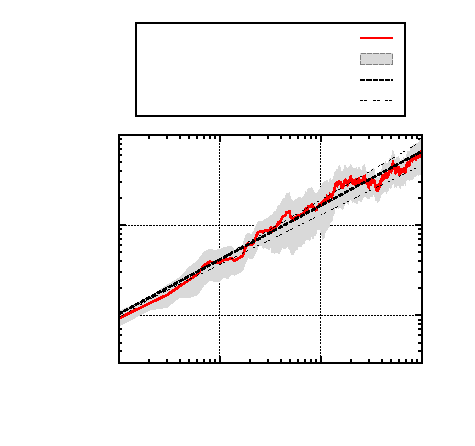
\includegraphics{MSD_error_s}}%
    \gplfronttext
  \end{picture}%
\endgroup

}}
\caption{Dubbellogplott av de olika sorternas MSD för celler i dvala med felgränser och möjliga anpassningar. De olika MSD:erna beräknades med \eqref{eq:MSD_S} respektive \eqref{eq:MSD_s}. Felgränserna är satta som konfidensintervall med 95\,\% konfidens. Med felgränserna syns att exponenten kan variera omkring $\pm 0,05$; detta visar sig också vara fallet för celler i log-fas.}
\label{fig:MSD_error}
\end{figure}
%\restoregeometry

Jämförs exponenterna i potensanpassningen mellan cellerna i dvala och log-fas, (a) respektive (b) i \figref{fig:MSD}, finns en viss skillnad. Exponenten för cellerna i dvala är $0,6$ mot log-fas-cellernas $0,8$. Med osäkerhetsgränser som i \figref{fig:MSD_error} syns att dessa värden på exponenterna själva får en osäkerhet på ungeför $\pm 0,05$. Även om \figref{fig:MSD_error} bara visar detta för partiklar från celler i dvala så gäller samma osäkerhet i exponenten för celler i log-fas.

Även med felgränserna i \figref{fig:MSD_error} för exponenterna syns dock att båda processerna ändå är exempel på subdiffusion. Alltså att partiklarnas MSD beror av tiden som ett potenssamband med exponent mindre än $1$. Subdiffusion är en avvikelse från klassiska brownsk rörelse, där exponenten enligt \eqref{eq:MSD_brown} ska vara $1$. 


I \figref{fig:MSD} syns att MSD:n från \eqref{eq:MSD_s} är som förväntat mer ojämn än den stationära då färre medelvärden tas. Vidare ser $S$ och $s$ ut att ha ungefär samma värde i samtliga fall. Detta beror på normeringen från avsnitt~\ref{sec:resultat-storleksberoende} som använts för att normera mot inensiteten. Men då det bara är lutnigen, i dubbellogplot, på MSD:n som är intressant så påverkas inte resultaten av vilka absoluta värden MSD:n har.






\section{Anisotropi i partikelrörelsen}
Om man misstänker att cellens inre struktur påverkar partikelrörelserna skulle eventuell anisotropi kunna ge ett bidrag till dessa. Alltså ifall det finns föredragna riktningar för partikeln att röra sig i. Ett sätt att undersöka detta är genom att betrakta koordinaternas kovariansmatris som är en matris med de olika koordinaternas statistiska andramoment:
\begin{equation}
C_{ij} = \frac{1}{N} \sum_{n=1}^{N} 
\left(r_i^{(n)}r_j^{(n)} -\bar{r}_i\bar{r}_j \right),
\end{equation}
där $r_i^{(n)}$ är den $i$:te koordinaten ($x$ eller $y$) i den $n$:te datapunkten och $\bar{r}_i$ är den $i$:te koordinatens medelvärde. På matrisform kan $C$ skrivas som
\begin{equation}\label{eq:C_matris}
C=
\begin{bmatrix} 
\ev{x^2}-\ev{x}^2 & \ev{xy}-\ev{x}\ev{y}\\
\ev{yx}-\ev{x}\ev{y} & \ev{y^2}-\ev{y}^2
\end{bmatrix}.
\end{equation}

Notera hur snarlik $C$ är med tröghetsmatrisen för en kropps olika tröghetsmoment som uppkommer i mekaniken. Och precis som i mekaniken kan man hitta två principalaxlar genom att ta fram dess egenvektorer och diagonalisera matrisen. I mekaniken svarar principalaxlarna mot de riktningar av rörelsemängdsmoment som är oberoende av rotation längs andra axlar. I de här statistiska sammanhangen finns det en liknande tolkning nämligen att principalaxlarna svarar mot de riktningar i cellen där rörelserna är oberoende av varandra. Egenvärdena i dessa två riktningarna svarar mot variansen i den oberoende koordinaten längs med den riktningen.

För att ur kovariansmatrisen få ut ett mått på hur isotropt partikeln rör sig kan man undersöka asymmetrimåttet~\cite{Rudnick_Asphericity1986}
\begin{equation}\label{eq:asph.}
    A_d=\frac{\sum_{j=1}^d\sum_{i<j} 
\ev{(\lambda_i-\lambda_j)^2} }{
(d-1) \ev{(\sum_{j=1}^d \lambda_j)^2}}
\end{equation}
i $d$ dimensioner, kallat \emph{asfärisitet}. Egenvärdena själva svarar som sagt mot variansen i de olika riktningarna, vilket motsvarar hur mycket partikeln har rört sig i respektive rikting. Hade positionerna varit helt isotropt fördelade så hade alltså $A=0$, om partikeln bara hade rört sig längs en linje blir istället $A=1$.
I två dimensioner förenklas \eqref{eq:asph.} till 
\begin{equation}\label{eq:asph._2D}
    A=\frac{\ev{(\lambda_1 - \lambda_2)^2}}{\ev{(\lambda_1 + \lambda_2)^2}}.
\end{equation}

\subsubsection{Tillämpning av asfärisiteten}
Man kan enkelt visa att egenvärdena till kovariansmatrisen i \eqref{eq:C_matris} uppfyller~\cite{Hong_asymmetri1998}
\begin{equation}
\begin{aligned}
\lambda_1+\lambda_2 
&= \ev{x^2}-\ev{x}^2+\ev{y^2}-\ev{y}^2 
\\
\abs{\lambda_1-\lambda_2} 
&=\sqrt{\left(
            \left(\ev{x^2}-\ev{x}^2\right)^2
            -\left(\ev{y^2}-\ev{y}\right)^2
        \right)^2 
        +4(\ev{xy}-\ev{x}\ev{y})^2
}.
\end{aligned}
\end{equation}
För en given fördelningsfunktion med ändliga moment blir det därmed nu möjligt att beräkna denna kvot teoretiskt.

För en obegränsad Wienerprocess i $d$ dimensioner fås~\cite{Rudnick_Asphericity1986}
\begin{equation} \label{eq:Asphericity_Brownian}
    A_d^\text{(Wierner)}=\frac{2(d+2)}{5d+4}.
\end{equation}
För två dimensioner blir $A_2^\text{(Wierner)}=\nicefrac{4}{7}$. Detta innebär att även långvariga slumpvandringar i snitt kommer att uppvisa viss anisotropi.

För fBm fås en formel i två dimensioner som gäller i gränsen där antalet mätpunkter blir mycket stort ~\cite{Hong_asymmetri1998}
\begin{equation} \label{eq:A_fBm}
A=2-
\frac{\frac{1}{2(H+1)^2}}{\frac{1}{2(H+1)^2}+\frac{2H+1}{4(4H+1)}-\frac{1}{4H+3}-\frac{\Gamma^2(2H+2)}{\Gamma(4H+4)}},
\end{equation}
där $H$ är Hurst parametern som karakteriserar rörelsen och $\Gamma$ är gammafunktionen. För $H=\nicefrac{1}{2}$ fås en vanlig brownsk rörelse med motsvarande  asymmetrimått $A=\nicefrac{4}{7}$ vilket stämmer överens med ekvation \eqref{eq:Asphericity_Brownian} för $d=2$. Samma värde fås även approximativt för CTRW-modellen \cite{Ernst_ACTRW2012} då denna rörelse vid varje tidsögonblick ser ut som brownsk rörelse. \todo[color=lime]{Kanske kan förklaras bättre?}

%Även http://iopscience.iop.org/article/10.1088/0305-4470/19/4/004/pdf



 
\subsection{Simulering och numerisk beräkning av asymmetrimått} 
\label{sec:sim_asym}
Istället för att bara direkt beräkna $A$ enligt \eqref{eq:asph._2D} för den undersökta datan och några olika modeller kan man också studera fördelningen av måttet 
\begin{equation}\label{eq:asym}
\mathcal{A} =
\frac{(\lambda_1 - \lambda_2)^2}{(\lambda_1 + \lambda_2)^2}.
\end{equation}
Här ska det dock påpekas att det inte går att få $A$ från  $\ev{\mathcal{A}}$ eftersom \eqref{eq:asph._2D} består av ett väntevärde i både täljare och nämnare. Eftersom $\mathcal{A}$ alltså skiljer sig så från $A$ går det heller inte lika enkelt att göra teoretiska beräkningar, vilket gör att fördelningen av $\mathcal{A}$ får undersökas med Monte Carlo-simuleringar.


%Eftersom en mätning bara kan bestå av ett ändligt antal datapunkter kan även en äkta, isotrop brownsk rörelse ge upphov till $\mathcal{A}>1$. Vidare är \emph{kvoten} mellan egenvärden inte linjär, vilket gör en teoretisk analys av fördelningarna mycket svår. För att ändå kunna säga något om den riktiga datan kan man ganska enkelt ta fram en fördelning för $\mathcal{A}$ för några olika modeller genom simulering. 

De modeller som testats är en vanlig Wienerprocess, en Wienerprocess med ett ''mätbrus'' pålagt och en Ornstein-Uhlenbeck-process. Tyvärr simulerades inte \todo{Om inte någon annan vill ta/har tagit sig an detta.}fBm och CTRW då dessa modeller är betydligt mer komplexa och behöver mer avancerade simuleringsalgoritmer. 
Från dessa processer samt från datan över partikelrörelsen erhölls olika värden på $A$ och fördelningar av $\mathcal{A}$. 


I Wienerprocessen simulerades partikelns position i varje ny tidpunkt genom att gå ett normalfördelat steg från positionen i den förra tidpunkten. Detta kan skrivas som
\begin{equation}\label{eq:sim_wiener}
x_{i+1} = x_i + \sigma_\text{steg}\delta 
\qcomma  \delta \sim N(0, 1)
\end{equation}
och där $x_1=0$. Sedan gör man samma sak för $y$. Eftersom $\mathcal{A}$ ger ett mått på hur mycket partikeln \emph{föredrar en viss riktning}, finner man att värdet på $\sigma_\text{steg}$ inte påverkar fördelningen -- så länge $\sigma_\text{steg}$ är samma för både $x$ och $y$. Detta blir uppenbart när man tänker på att \eqref{eq:sim_wiener} kan skrivas som 
\begin{equation}
x_{i+1} =\sigma_\text{steg}\,x'_{i+1} = \sigma_\text{steg}\left( x'_i + \delta \right) 
\end{equation}
Alltså att $\sigma_\text{steg}$ bara är en multiplikativ konstant framför positionen.

För att istället simulera en Wienerprocess med mätbrus användes \eqref{eq:sim_wiener} för att först simulera själva Wienerprocessen för att sedan \emph{efteråt} addera en slumpad brusterm $\sigma_\text{brus}\eta$ till varje position $x_i$. Positionerna i simuleringen med brus ges alltså av
\begin{equation}
\hat{x}_{i} = x_i + \sigma_\text{brus}\eta 
\qcomma  \eta \sim N(0, 1).
\end{equation}
Den väsentliga skillnaden mot en ren Wienerprocess är att mätbruset $\eta$ inte påverkar nästkommande position. Till skillnad från den rena Wienerprocessen så kommer värdena på $\sigma_\text{steg}$ och $\sigma_\text{brus}$ att påverka $\mathcal{A}$, men enligt samma argument som ovan kommer bara kvoten $\nicefrac{\sigma_\text{brus}}{\sigma_\text{steg}}$ vara det som påverkar. Detta gör att simuleringarna med mätbrus går att genomföra med olika värden på parametern $\nicefrac{\sigma_\text{brus}}{\sigma_\text{steg}}$ för att få olika fördelningar av~$\mathcal{A}$. 

Ornstein-Uhlenbeck-processen i \eqref{eq:SDE_o-u} simulerades genom att använda derivatan för tidsutveckling och genom att sätta $\bar{x}=0$. Man får då
\begin{equation}
x_{i+1} = x_i + \Delta{t}\,\pd_{t}x  = (1-k) x_i +  \sigma_\text{steg}\delta 
\qcomma  \delta \sim N(0, 1),
\end{equation}
där $x_1=0$. Notera här att den styrande parametern i simuleringarna är $k=\gamma\Delta{t}$, samt att $\sigma_\text{steg}$ på samma sätt som för den rena Wienerprocessen kan väljas godtyckligt utan att påverka $\mathcal{A}$. 

Samtliga simuleringar har gjorts med 1000 steg och 100\,000 upprepningar. Antalet steg valdes för att simuleringarna ska efterlikna den studerade datan -- som består av 1000 sparade positioner för varje partikel. Däremot kan upprepningarna väljas godtyckligt. Då valdes 100\,000 för ge tillräckligt jämna fördelningar.\todo{Borde man flytta det här till resultatet?}

%Vill Emelie lägga in något resultat om detta så får hon gärna lägga tillbaks det här stycket
%Eftersom resultatet för asymmetrimåttet i ekvation \eqref{eq:A_fBm} gäller för riktigt långa mätningar medan den data som analyseras i detta arbete är ganska begränsad kan man försöka simulera fram sannolikheter istället. Genom att simulera många mätserier för samma antal steg och antal partiklar som i datan kan man bedöma sannolikheten att det framräknade asymmetrimåttet till exempel skulle ha kommit från en ren klassisk brownsk rörelse. 


\subsection{Resultat -- partikelrörelserna är isotropa och behöver inte delas upp i anpassade koordinater}
\label{sec:resultat-isotropi}

\begin{figure}\centering
\input{bilder/partiklar/isotropi_asymmetri.tex}
\caption{Fördelning av asymmetrimåttet $\mathcal{A}$ enligt \eqref{eq:asym}, visat som sannolikheten att $\mathcal{A}$ är \emph{större} än ett visst värde $a$.
Graferna visar att de partiklar från celler i log-fas, i det här avseendet, beter sig som en Wiernerprocess. Partiklarna från celler i dvala beter sig däremot mer isotropt än en vanlig Wienerprocess; deras betende skulle kunna modelleras som en Wienerprocess med pålagt brus med $\nicefrac{\sigma_\text{brus}}{\sigma_\text{steg}} = 6$ eller som en Ornstein-Uhlenbeck-process med tidskonstant $\nicefrac{1}{\gamma} =\unit[4]{s}$.
}
\label{fig:asymmetri}
\end{figure}

\begin{table}
\centering
\caption{Värden på asfärisitetsen $A$ enligt \eqref{eq:asph._2D} för de undersökta partiklarna och processerna. De simulerade värden kommer från simuleringarna gjorde med 1000 steg och 100\,000 upprepningar med samma parametrar som i \figref{fig:asymmetri}. De små osäkerheterna i de simulerade värdena beror på att medelvärdena kommer från så många simuleringar. Osäkerheterna i de angivna värdena är angivna med en standardavvikelse. 
%Läsaren påminns om att en helt cirkulärt symmetrisk fördelning svarar mot $\mathcal{A}=0$, medan $\mathcal{A}=1$ svarar mot att positionerna ligger på en linje.
}
\label{tab:asph._values}
\begin{adjustbox}{center}
\begin{tabular}{l|c|c|c|c|c|c|}\cline{2-7}
%första raden
& \multicolumn{2}{c|}{Uppmätta} 
& Teoretisk 
& \multicolumn{3}{c|}{Simulerade}
\\ \cline{2-7}
%Första delen av andra raden
& \multirow{3}{*}{Log-fas} & \multirow{3}{*}{Dvala }%mätdata
& \multicolumn{3}{c|}{Wienerprocesser }%Wiener 
& 
\\ \cline{4-7}%\cline{2-3}\cline{6-7}
& & & \multicolumn{2}{c|}{\multirow{2}{*}{utan mätbrus} }%Wiener
& med mätbrus  & O-U-process %simulerade brus och O-U
\\
%Andra delen av andra raden
& & &\multicolumn{2}{c|}{}
& $\nicefrac{\sigma_\text{brus}}{\sigma_\text{steg}} = 6$ & $\nicefrac{1}{\gamma} =\unit[4]{s}$
\\\hline
%Sista raden, med värden
\multicolumn{1}{|l|}{$A$:}
& $0,41\pm 0,23$ & $0,49\pm 0,15$ %mätdata
& $\nicefrac{4}{7}\approx 0,571$ & $0,570\pm 0,005$ %Wiener
& $0,43\pm 0,003$ & $0,34\pm 0,002$ %brus och O-U
\\ \hline
\end{tabular}
\end{adjustbox}
\end{table}

\todo[color=lime]{Ska vi säga något om att banorna verkade vara like assymetriska?}
Som kan ses i \figref{fig:asymmetri} skiljer sig den simulerade asfärisiteten $\mathcal{A}$ mellan partiklar från celler i dvala och de i log-fas. Båda fallen har fördelningar som svarar mot en rörelse som är minst lika isotrop som Wiernerprocessen -- under de undersökta tidsskalorna. Vidare ses att partiklarna från celler i dvala får en fördelning av $\mathcal{A}$ med betydligt lägre sannolikhet för högre $\mathcal{A}$-värden, svarande mot mer asymmetriska rörelser. Skillnaden mellan cellfaserna tyder på att något förändras i cytoplasman när cellen går i dvala, något som påverkar partikelrörelserna. 

Om istället det riktiga asfärisitetsmåttet, $A$ från \eqref{eq:asph._2D}, betraktas erhålls värdena i \tabref{tab:asph._values} där uppmätta, teoretiska och simulerade värden presenteras med felgränser. Det bör dock nämnas att det teoretiska värdet gäller i gräns mot när antalet steg går mot oändligheten medan de simulerade och uppmätta värdena beräknats från diskreta datamängder. Viss avvikelse kan därför vara att vänta. Från tabellen ses att de uppmätta värdena på $A$ för partiklarna, $0,41\pm0,23$ för log-fas och $0,49\pm0,15$ för cellerna i dvala, på grund av sin stora felgräns omsluter både resultatet för Wienerprocessen och O-U-processen med tidskonstant $\nicefrac{1}{\gamma}=\unit[4]{s}$. Partikelrörelsen är alltså minst lika isotrop som dessa båda processer.

\section{PSD}



%Lite om hur det borde se ut om det var brownsk
Som sagts i avsnitt~\ref{sec:white_noise} så beskriver Wiernerprocessen brownsk rörelse matematiskt. Detta gör att Man kan få PSD:n för brownsk rörelse genom att undersöka Wiernerprocessen. En sak som också nämndes i avsnitt~\ref{sec:white_noise} är att Wienerprocessen kan tolkas som \emph{integralen av vitt brus}. Så PSD:n för Wienerprocessen kan alltså uttryckas med hjälp av den konstanta PSD:n för vitt brus.
På ett lite handviftande vis bör alltså 
\begin{equation}
S_\text{Wiener} (f) \propto f^{-2} S_\text{Vitt brus}(f) \propto f^{-2}.
\end{equation}
Här har man utnyttjat PSD:ns koppling till Fouriertransformen, så att integrering kan skrivas som att transformen multipliceras med $(\ii f)^{-1}$. Sedan följer kvadraten av att PSD använder beloppskvadraten av transformen. 

\subsection{Resultat -- }


\section{Diskussion}
\todo[inline]{Inga tomma rubriker}


\subsection{MSD -- subdiffusivt beteende pekar mot att vanlig brownsk rörelse inte räcker som förklaringsmodell}
%Klippt från resultatdelen
Då MSD:n ger en vink om hur snabbt partiklarna sprids verkar partiklarna i cellerna i dvala diffundera långsammare än partiklarna i de aktiva cellerna. De undersökta cellernas metabola tillstånd verkar alltså påverka diffusionen i cytoplasman vilket bekräftar resultat från tidigare studier~\cite{Parry_etal2014}. Dessa studier har, liksom här, utförts på celler utan motorprotein. Detta utesluter förklaringsmodellen där de utpekas som största bidragsfaktor som möjlig förklaring det det observerade fenomenet. 




%\subsection{Intensitetskorrigering}

\subsection{Brusnivån är lägre än väntat}
Som resultaten i avsnitt~\ref{sec:resultat-storleksberoende} visar är brusnivån ganska låg, omkring \unit[5]{nm}. Detta är är lågt, vilket skulle kunna tyda på att metoden är bristfällig.

För det första kan det kännas märkligt att ens kunna prata om observationer av nanometerstora röreler gjorda med ett \emph{optiskt} mikroskop. Instinktivt borde det inte gå att upplösa något som är mindre än ljusvåglängden, på flera hundra nanometer. Och om inte ljusets våglängd skulle vara begränsande, så borde i alla fall bildsensorns pixelstorlek sätta en nedre gräns i upplösningen. Men så är faktiskt inte fallet. Det går att få subpixelnoggannhet~\cite{Saunter2010} genom att utnyttja olika databehandlignstekniker som hittar centrum på en flera pixlar bred ljusfäck på kamerasensorn.

Med detta sagt behöver man dock komma ihåg att sådan subpixelnoggrannhet typiskt ger en maximal upplösning på omkring en tiondels pixel~\cite{Saunter2010}. I det här fallet skulle detta svara mot cirka 11\,nm upplösning. Detta är också den brusnivå som \cite{Midtveldt_etal2016} kom fram till när de analyserade samma data. De använde sig dock av en metod där de undersökte partiklarnas PSD för att hitta en brusbakgrund. 


Från \figref{fig:storleksberoende}, framför allt (c) och (d), kan man dock se att $\sigma_\text{brus}=\unit[11]{nm}$ verkar vara en överskattning. För om den faktiska brusnivån var \unit[11]{nm} så borde väldigt få mätpunkter hamna under den utmarkerade linjen för \unit[11]{nm}-brus i \figref{fig:storleksberoende}. Detta verkar endast vara fallet för log-fas i \figref{fig:storleksberoende}~(b), men tittar man på steglängderna i log-fas (d) så går de ner under \unit[11]{nm}-nivån.

Avslutningsvis bör dock också sägas att brusnivån på cirka \unit[5]{nm} kan vara lite i lägsta laget. Detta för att ju högre intensitet en partikel har, desto lättare blir det att lokalisera den i ett mikroskop. Och eftersom brusnivån i den här studien beräknades från de partiklar med högs intensitet, så kan det hända att den uppmätta mätosäkerheten blir lägre här för att den är lägre för de större partiklarna. Dock verkar ändå \unit[5]{nm} vara den bättre uppskattningen.





\subsection{Isotropi}

En anledning att studera isotropin är att bedöma hurvida det finns en föredragen rikting i cellerna. Hade så varit fallet hade $A$ varit större för partiklarna än för Wienerprocessen. Detta skulle i så fall antyda om att det skulle finnas strukturer i cellen som påverkar partikelrörelsen. Det skulle då vara befogat att studera rörelserna längs dessa föredragna riktingar separat genom att till exempel införa normal- och tangentialkoordinater. Från avsnitt~\ref{sec:resultat-isotropi} visar sig dock detta \emph{ej} vara fallet.

Genom att gå över till normal och tangentialkoordinater när detta inte är motiverat riskerar att leda till metodfel i dataanalysen. Ett sådant koordinatbyte kan leda till att man hittar mönster som egentligen inte finns men som normaltsett uppstår, även i vanlig brownsk rörelse. En stark motivering bör därför föregå ett sådant koordinatbyte. Eftersom det inte finns några indikationer på att det skulle finnas en strukturell anisotropi har inga sådana koordinatbyten gjorts i den här studien.


En annan anmärkningsvärd sak är att de olika asymmetrimåtten skiljer sig så tydligt åt mellan cellfaserna. Fördelningen av $\mathcal{A}$ från \figref{fig:asymmetri} tyder på att partiklar från celler i dvala beter sig mer isotropt, medan värden på $A$ i \tabref{tab:asph._values} pekar på ett överlapp mellan partiklar från celler i dvala eller log-fas. Det är till och med så att värden i \tabref{tab:asph._values} eventuellt antyder om att partiklar från celler i log-fas beter sig mer isotropt, men det är för stora felmarginaler för att kunna dra några slutsatser.

\subsubsection{Mätbrus är ingen tillfredsställande förklaring}
Förhållandet mellan standardavvikelsen för bruset och steglängden $\nicefrac{\sigma_\text{brus}}{\sigma_\text{steg}}$ varierade i den undersökta datan på grund av olika rörlighet för olika partiklar. Större partiklar tenderade att förflytta sig kortare sträckor än de små partiklarna. Från beräkningarna av medelstegen i \figref{fig:storleksberoende}~(c) och (d) visade det sig också att medelstegens standardavvikelse var omkring $\unit[10\pm 5]{nm}$. Vilket, med $\sigma_\text{brus}=\unit[5]{nm}$ från avsnitt~\ref{sec:resultat-storleksberoende}, skulle svara mot $\nicefrac{\sigma_\text{brus}}{\sigma_\text{steg}}=0.5\pm 0.2$. Det verkar alltså högt osannolikt att isotropin för partiklar i celler i dvala skulle kunnat ha uppstått från så brusig data som användes i avsnitt~\ref{sec:resultat-isotropi}. 

En annan anledning att brusig data inte kan förklara avvikelsen för celler i dvala i \figref{fig:asymmetri}, är att pertiklarna från celler i log-fasen inte påverkades trots att brusnivån borde vara samma i båda fallen. Man skulle kunna argumentera för att $\nicefrac{\sigma_\text{brus}}{\sigma_\text{steg}}$ ändå kan skilja sig mellan de olika cellfaserna för att $\sigma_\text{steg}$ skulle kunna variera. \figref{fig:storleksberoende}~(c) och (d) visar dock tydligt hur steglängderna mer eller mindre är de samma mellan cellfaserna.

Hypotesen, att mätbrus skulle kunna förklara avvikelserna från brownsk rörelse, kan alltså förkastas även då värdena för asfäriteten i \tabref{tab:asph._values} och dess fördelnigen \figref{fig:asymmetri} ser ut att kunna stämma. 

Den andra förklaringsmodellen, Ornstein-Uhlenbeck-processen, diskuteras vidare i dess egna avsnitt längre ner. För tillfället räcker det att säga att den är mer tillfredsställande än brusmodellen. 



\subsubsection{Inget intensitetsberoend i asymmetrin pekar mot storlekoberoende partikelbindning}
I isotropimätningarna användes ingen intensitetskorrigering. Den huvudsakliga anledningen till detta var att oavsett hur stora partiklarna är så borde de ändå ha samma rörlighet i olika riktningar. Man skulle dock kunna invända mot detta genom att mena att en större partikel skulle vara hårdare bunden. Detta skulle motsvara en mindre tidskonstant i en Ornstein-Uhlenbeck-modell, vilket skulle ha gett mer isotropa fördelningar för större partiklar.

När man undersöker om det finns något beroende mellan $\mathcal{A}$ och partikelintensiteten, så finner man dock ingen tydlig trend. Detta gäller oavsett vilken cellfas som undersöks.
Intensitetsoberoendet här verkar alltså peka mot att olika stora partiklar ändå har samma bindningsstyrka i en Ornstein-Uhlenbeck-modell. 



%Om sambandet mellan intensitet och partikelstorleken påverkar resultatet

%Byter man till normal- och tangential-koordinater bygger man in ett bias som påverkar resultaten till att det verkar finnas egenskaper som egentligen inte finns. 
%Av slumpskäl kommer vissa vägar att vara mer raka än andra medan andra får mer symmetriska banor.



\subsection{Ornstein-Uhlenbeck-modellen kan inte förklara subdiffusion men skulle kunna användas i andra sammanhang}

Notera att för $\gamma\Delta{t}\ll 1$ så ger \eqref{eq:MSD_o-u} att 
$\ev{(x(t)-x(t') )^2}\widetilde{\propto}\,\Delta{t}$. Detta betyder alltså att Ornstein-Uhlenbeck-processen inte kan användas för att förklara tidigare observerade avvikelser\cite{Hofling&Franosch2013} i partiklars MSD. Dock så är den här modellen bara en första utveckling av brownsk rörelse, så det är inte så förvånane att den inte skulle klara av att förklara allt. Men förhoppningsvis skulle den kunna förklara vissa beteenden som observeras. 


\subsubsection{Modell för att förklara skillnad i isotropi mellan cellfaserna}



\subsection{Uppskattning av Hurstparametern och fBm som modell för partikelrörelse i celler}

Då Hurstparametern för en fBm återfinns i många förutsägelser för rörelsen kan denna uppskattas från flera håll, bland annat från exponenten i MSD:n \eqref{eq:fBm_MSD} och som parameter i asfärisiteten \eqref{eq:A_fBm}. 
I figur \figref{fig:MSD} presenterades värdena för MSD:n för datan till att vara $0,65\pm0,01$ för cellerna i dvala och $0,80\pm0,05$ för log-fas cellerna. Detta svarar via \eqref{eq:fBm_MSD} mot $2H$ vilket ger $H=0,325\pm0,005$ och $H=0,40\pm0,03$ för cellerna i dvala respektive log-fas cellerna.
Beräknade värden för asfärisiteten presenteras i tabell \tabref{tab:asph._values}. För cellerna i dvala fås $H=0,41\pm 0,23$ och för log-fas cellerna $H=0,49\pm 0,15$. Motsvarande H-värde fås approximativt från \eqref{eq:A_fBm} till att bli $H=0,36\pm0,20$ respektive $H=0,43\pm0,13$, om relativa felet bevaras. Snitten mellan de två uppskattningarnas intervall är nollskilda för respektive cellfas vilket ger viss rimlighet till fBm som modell för partikelrörelse i celler. Den stora felgränsen i uppskattningen av H från asfärisiteten gör dock detta påstående svagt.

Båda dessa uppskattningar av $H$ ger ett värde som med stor sannolikhet befinner sig under $\nicefrac{1}{2}$, svarande mot en rörelse med positiv korrelation mellan två positioner i rörelsen, dvs att partikeln tenderar att röra sig bort från startpositionen. Detta kan vara ett rimligt resultat under de tider som studeras här då cellens begränsade utbredning inte begränsar rörelsen. För längre samplingstider skulle man dock kunna förvänta sig $H>\nicefrac{1}{2}$, där negativ korrelation fås i rörelsen och partikeln tenderar att röra sig tillbaka mot startpositionen. 

Som modell skulle fBm med ovanstående beräkningar nog kunna beskriva vissa egenskaper hos partikelrörelse i celler, åtminstone approximativt. Modellen ger dock inte någon fysikalisk beskrivning till rörelsens egenskaper utan bara matematiska förutsägelser. Denna avsaknad av koppling mellan den mikroskopiska, underbyggande fysiken och de makroskopiska, observerade egenskaperna gör fBm mindre tilltalande som kandidat för den alltäckande modellen för partikelrörelse i celler. Vidare studier på partikelrörelse i jästceller skulle kunna bekräfta fBm:s användbarhet som matematisk modell, men som fysikalisk modell brister den i sin avsaknad av tydlig fysikalisk tolkning.
\todo[color=lime]{Ska vi vara så här ärliga?}

\subsection{Något om CTRW}
Stationär process $->$ CTRW inte så aktuell.

\todo[color=lime,inline]{Ska vi säga något om CTRW som modell här?}

%Bara en liten kodsnutt som behövs när man kompilerar lokalt
%%% Local Variables: 
%%% mode: latex
%%% TeX-master: "00main.tex"
%%% End: 